% Created 2020-01-09 jeu. 14:38
% Intended LaTeX compiler: pdflatex
\documentclass[11pt]{article}
\usepackage[utf8]{inputenc}
\usepackage[T1]{fontenc}
\usepackage{graphicx}
\usepackage{grffile}
\usepackage{longtable}
\usepackage{wrapfig}
\usepackage{rotating}
\usepackage[normalem]{ulem}
\usepackage{amsmath}
\usepackage{textcomp}
\usepackage{amssymb}
\usepackage{capt-of}
\usepackage{hyperref}
\usepackage{minted}
\author{Q. MARTY et P. POMERET-COQUOT}
\date{Automne 2019}
\title{T.P. Simulation (S.M.A.)}
\hypersetup{
 pdfauthor={Q. MARTY et P. POMERET-COQUOT},
 pdftitle={T.P. Simulation (S.M.A.)},
 pdfkeywords={},
 pdfsubject={},
 pdfcreator={Emacs 25.2.2 (Org mode 9.2.4)}, 
 pdflang={English}}
\begin{document}

\maketitle

\section{Introduction}
\label{sec:org9b3f6ac}

Les commerces en ville se situent généralement autour des grands axes,
dans une situation de forte concurrence.

La simulation que nous proposons se base sur l'hypothèse que cette répartition
s'explique par le seul comportement de la clientèle. 
Nous arrivons à reproduire ce mécanisme.

La section 2 présente notre cas d'étude. 
La section 3 résume les choix de modélisation détaillés dans la fiche \emph{ODD}. 
La section 4 expose nos résultats et constatations.
La conclusion est en section 5.

\section{Cas d'étude}
\label{sec:org33fbf51}

Nous nous intéressons à la localisation des commerces concurrentiels en ville.

Nous avons observé in-situ que les commerces sont principalement situés sur les axes de passage,
et que les commerces proches proposent souvent des services identiques.

Nous souhaitons simuler ces comportements sur des données réelles, et dans le cas de données
modifiées (ajout d'un arrêt de bus par exemple).

Nous travaillons d'abord sur la \emph{route de Narbonne} (Toulouse) et les rues environnantes (figure \ref{fig:orga17fbd9}),
puis vérifions si nous obtenons des résultats similaires sur d'autres quartiers.

\section{Choix de modélisation}
\label{sec:org2269d5b}
La fiche \emph{ODD} accompagnant ce rapport donne les détails de la modélisation.
Nous reprenons ici les grandes lignes.


\begin{figure}[htbp]
\centering
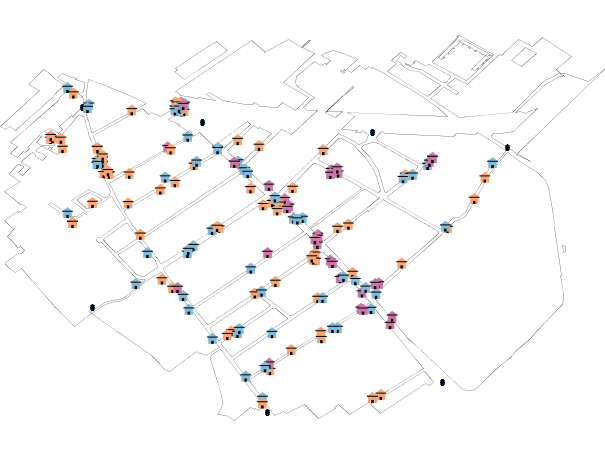
\includegraphics[width=200px]{./images/t=0.png}
\caption{\label{fig:orga17fbd9}
État initial du système}
\end{figure}

\subsection{Le monde}
\label{sec:orga770fad}
Les rues (\emph{roads}) sont les seuls patches accessibles du monde. 
Nous utilisons les données du cadastre pour les identifier.

Certains patches de rue sont des puits (\emph{wells}), qui servent d'entrée et de
sortie pour les clients. Ces puits sont placés manuellement sur la carte (avec QGis)
aux extrémités des rues, et possèdent un poids représentant leur fréquentation.

\subsection{Les boutiques}
\label{sec:org2c4b9e2}
\subsubsection{Représentation}
\label{sec:orgfe5f0d1}
Les boutiques possèdent une position, un domaine d'activité (\emph{market}) représenté par leur couleur, des fonds (\emph{funds}) représentés par leur taille,
et une file d'attente (\emph{queue}).
\subsubsection{Initialisation}
\label{sec:orgaff91d2}
Les boutiques sont générées d'après la base Sirene : leur position et leur domaine
d'activité est réaliste. Toutes commencent avec la même somme d'argent et une file d'attente vide (figure \ref{fig:orga17fbd9})
\subsubsection{Comportement}
\label{sec:org7a1dd72}
Les boutiques gagnent 1 sou lorsqu'un client y consomme, et en perdent lorsqu'un
client est généré. Cela nous permet de simuler une taxe qui est exactement égale
à l'argent gagné par les commerces, afin de conserver un niveau constant d'argent en circulation.

A chaque client, la file d'attente grandit, elle réduit à chaque tick.

De plus, si une boutique prospère (deux fois ses fonds de départ), alors elle
finance un nouveau commerce voisin de même type.

\subsection{Les clients}
\label{sec:orgf51a887}
\subsubsection{Représentation}
\label{sec:orgc2882de}
Les clients possèdent de l'argent (\emph{money}), 
un besoin  (\emph{need}) correspondant à un domaine d'activité des boutiques
et une destination (l'un des puits).
\subsubsection{Initialisation}
\label{sec:org1807c5d}
Les clients commencent sur un puits, avec un besoin et une destination (choisis au hasard pondéré). 
Initialement, ils possèdent tous la même quantité d'argent (\emph{base-money}).
\subsubsection{Comportement}
\label{sec:orgb0e556f}
Un client consomme s'il passe à proximité d'une boutique
adaptée, où l'attente est raisonnable. Il donne alors 1 sou à la boutique.

Un client atteignant sa destination disparaît, et un autre client est alors généré.
Cela assure une population constante.

\section{Résultats de la simulation}
\label{sec:org8387a80}

Après stabilisation du système (figure \ref{fig:orgde578a5}), nous observons la répartition
géographique des commerces.
Dans tous les cas suivants, les commerces s'agglomèrent par type 
(comportement émergent issu des faillites et créations successives).


\begin{figure}[htbp]
\centering
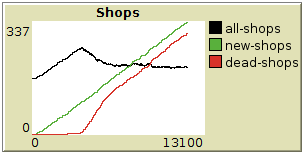
\includegraphics[width=140px]{./images/shop_count.png}
\caption{\label{fig:orgde578a5}
Stabilisation du système : les commerces se créent à la même vitesse qu'ils font faillite (leur nombre est constant)}
\end{figure}

Avec une seule consommation par client (\emph{base-money} = 1), et une vitesse
d'écoulement de la file d'attente raisonnable (\emph{queue-speed} = 0.1), 
les commerces se regroupent autour des puits (figure \ref{fig:org17d447f}).

\begin{figure}[htbp]
\centering
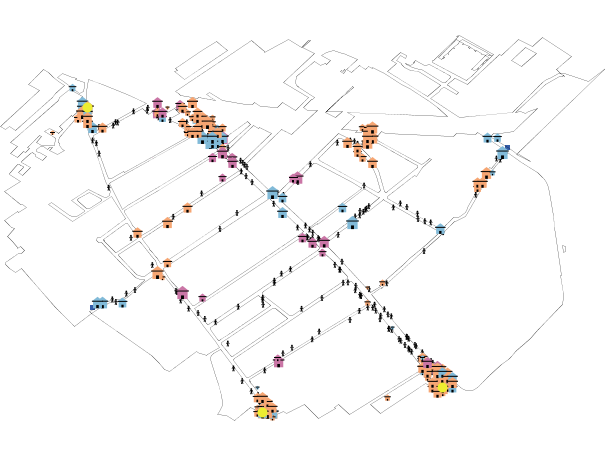
\includegraphics[width=150px]{./images/t=12000_base-money=1_patience=10_queue-speed=0.5_maxdd=5.png}
\caption{\label{fig:org17d447f}
Les clients consomme une seule fois}
\end{figure}


Avec plusieurs consommations par clients (\emph{base-money} = 3) ou une
vitesse d'écoulement de la file d'attente très faible (\emph{queue-speed} = 0.01),
les clients sont poussés à consommer plus loin, et les commerces se 
répartissent alors sur les axes principaux (figure \ref{fig:orgfecf45f})

\begin{figure}[htbp]
\centering
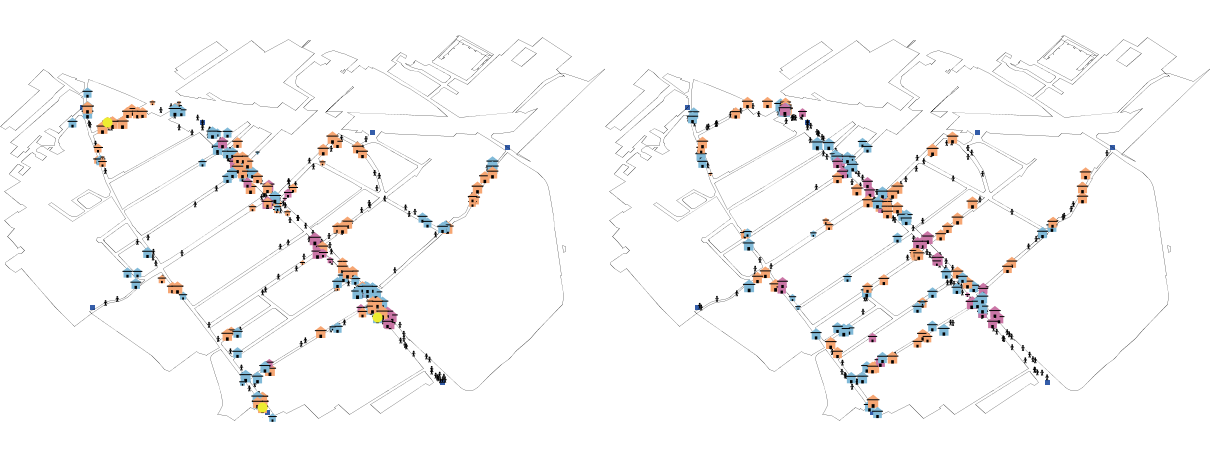
\includegraphics[width=300px]{./images/grands_axes.png}
\caption{\label{fig:orgfecf45f}
Les clients consomment 3 fois (à gauche), ou l'écoulement des files d'attentes est lent (à droite)}
\end{figure}

\section{Conclusion}
\label{sec:orgc165a4c}

Avec ce super modèle on peut bien s'amuser :-)
\end{document}
